\documentclass[12pt]{article}
\usepackage{
  amsmath,
  booktabs,
  enumitem,
  geometry,
  graphicx,
  microtype,
  parskip,
}
\geometry{margin=3cm}

% meta data
\newcommand{\chapter}{2.4}
\newcommand{\authorname}{Amo DelBello}
\newcommand{\classdescription}{MATH 1350-D2}
\newcommand{\classname}{Introduction to Statistics, Fall 2022}
\newcommand{\assignment}{\chapter\ Book Assignment}

\newcommand{\problem}[1]{\vspace{5ex}\section*{\chapter-#1}}
\newcommand{\thead}[1]{\textnormal{\textbf{#1}}}
\newcommand{\tvspace}{\vspace{.25cm}}

\title{\classdescription\ \\ \classname\ \\ $\ $ \\ \assignment}
\author{\authorname}
\date{\today}


\begin{document}
\maketitle

\problem{1}
We refer to it as linear because it is a straight line. It measures the strength of the \textit{linear} association between two variables.


\problem{2}
No, we cannot conclude that gaining weight is a cause of increased blood pressure because \textit{correlation does not imply causation}.


\problem{3}
A scatterplot is a plot of paired (x,y) quantitative data with a horizontal x-axis and a vertical y-axis. It helps us to visually determine whether there is a correlation between two variables.


\pagebreak
\problem{5}
\begin{figure}[ht]
  \centering
  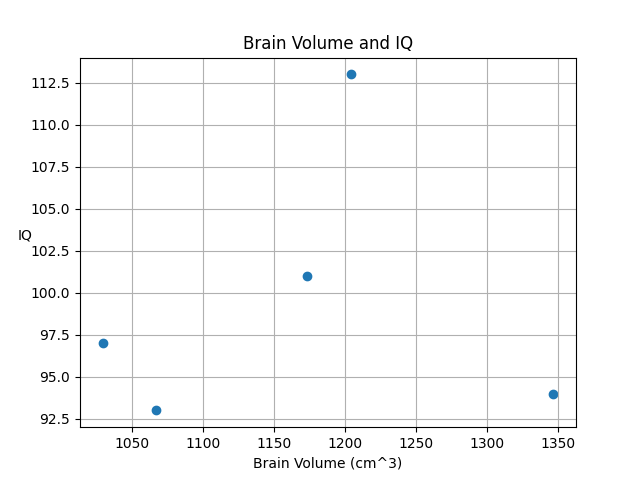
\includegraphics[width=12cm]{assets/brain-volume-and-iq.png}
  \caption{Brain Volume and IQ}
\end{figure}

There does not appear to be any correlation between brain density and IQ.\


\pagebreak
\problem{8}
\begin{figure}[ht]
  \centering
  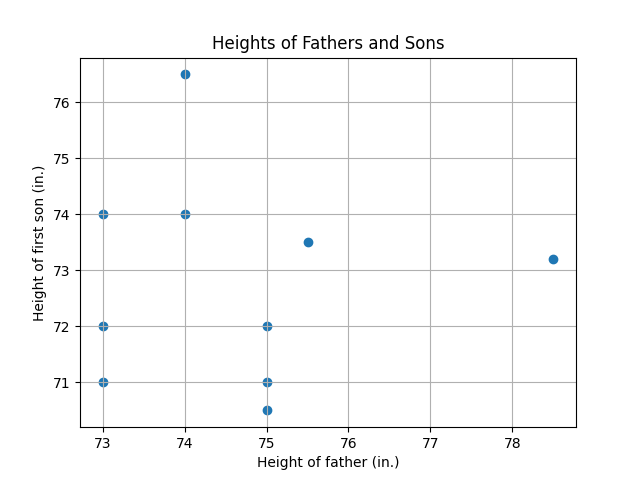
\includegraphics[width=12cm]{assets/heights-of-fathers-and-sons.png}
  \caption{Heights of Fathers and Sons}
\end{figure}

There does not appear to be any correlation between the heights of fathers and their first born sons.


\problem{9}
$r = 0.127$ and the critical values of $r$ with 5 data points are -0.878, 0.878. The $r$ value falls in-between the critical values. Therefore there \textit{is not a linear correlation} between brain volume and IQ.\


\problem{10}
$r = 0.980$ and the critical values of $r$ with 7 data points are -0.754, 0.754. The $r$ value falls outside the critical values. Therefore there \textit{is a linear correlation} between chest sizes and weights in anesthetized bears.


\problem{11}
$r = -0.987$ and the critical values of $r$ with 7 data points are -0.754, 0.754. The $r$ value falls outside the critical values. Therefore there \textit{is a linear correlation} between car weight and fuel consumption.


\problem{12}
$r = -0.017$ and the critical values of $r$ with 10 data points is -0.632, 0.632. The $r$ value falls in-between the critical values. Therefore there \textit{is not a linear correlation} between the heights of fathers and their first born sons.


\end{document}
%%% Local Variables:
%%% mode: latex
%%% TeX-master: t
%%% End:
